
% =============================================================================
% Figure 01 — Invariance and Transformation
% Book I — Ontology of Viability
% Chapter 02 — Invariance
%
% Purpose:
%   To illustrate the relation between an existent, a transformation,
%   and the possible preservation or alteration of determinations
%   and relations across that transformation.
%
% Conceptual Policy:
%   1. Invariance is not identical to identity.
%   2. Transformation does not necessarily eliminate invariance.
%   3. Invariance is assessed relative to a specified domain
%      and respect of transformation.
%   4. The existence of an invariant is not presupposed.
%   5. Invariance does not imply immutability or total preservation.
%
% Dependencies:
%   TikZ (already loaded in the project preamble)
%
% =============================================================================

\begin{figure}[htbp]
    \centering

    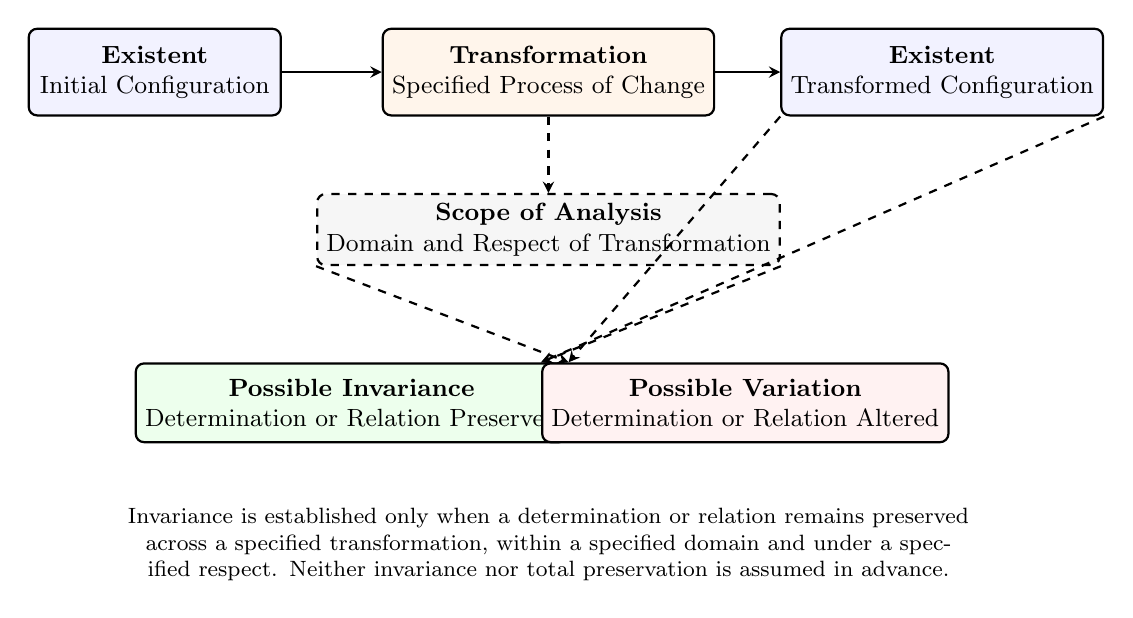
\begin{tikzpicture}[
        font=\small,
        existent/.style={
            draw,
            rounded corners=3pt,
            thick,
            minimum width=3.2cm,
            minimum height=1.1cm,
            align=center,
            fill=blue!5
        },
        transformation/.style={
            draw,
            rounded corners=3pt,
            thick,
            minimum width=3.0cm,
            minimum height=1.1cm,
            align=center,
            fill=orange!8
        },
        invariant/.style={
            draw,
            rounded corners=3pt,
            thick,
            minimum width=4.0cm,
            minimum height=1.0cm,
            align=center,
            fill=green!7
        },
        changing/.style={
            draw,
            rounded corners=3pt,
            thick,
            minimum width=4.0cm,
            minimum height=1.0cm,
            align=center,
            fill=red!5
        },
        condition/.style={
            draw,
            rounded corners=3pt,
            dashed,
            thick,
            minimum width=5.0cm,
            minimum height=0.9cm,
            align=center,
            fill=gray!7
        },
        mainarrow/.style={
            ->,
            thick,
            >=stealth
        },
        possiblearrow/.style={
            ->,
            thick,
            dashed,
            >=stealth
        }
    ]

    % -------------------------------------------------------------------------
    % Main sequence: initial configuration, transformation, resulting state
    % -------------------------------------------------------------------------

    \node[existent] (initial) at (0,0) {
        \textbf{Existent}\\
        Initial Configuration
    };

    \node[transformation] (transform) at (5.0,0) {
        \textbf{Transformation}\\
        Specified Process of Change
    };

    \node[existent] (result) at (10.0,0) {
        \textbf{Existent}\\
        Transformed Configuration
    };

    \draw[mainarrow] (initial.east) -- (transform.west);
    \draw[mainarrow] (transform.east) -- (result.west);

    % -------------------------------------------------------------------------
    % Analytical scope
    % -------------------------------------------------------------------------

    \node[condition] (scope) at (5.0,-2.0) {
        \textbf{Scope of Analysis}\\
        Domain and Respect of Transformation
    };

    \draw[possiblearrow] (transform.south) -- (scope.north);

    % -------------------------------------------------------------------------
    % Possible preservation and possible alteration
    % -------------------------------------------------------------------------

    \node[invariant] (preserved) at (2.5,-4.2) {
        \textbf{Possible Invariance}\\
        Determination or Relation Preserved
    };

    \node[changing] (changed) at (7.5,-4.2) {
        \textbf{Possible Variation}\\
        Determination or Relation Altered
    };

    % Analytical possibilities arising in relation to the transformed state.
    \draw[possiblearrow] (result.south west) -- (preserved.north east);
    \draw[possiblearrow] (result.south east) -- (changed.north west);

    % The scope of analysis conditions both assessments.
    \draw[possiblearrow] (scope.south west) -- (preserved.north east);
    \draw[possiblearrow] (scope.south east) -- (changed.north west);

    % -------------------------------------------------------------------------
    % Explanatory note
    % -------------------------------------------------------------------------

    \node[
        text width=11.5cm,
        align=center,
        font=\footnotesize
    ] (note) at (5.0,-6.0) {
        Invariance is established only when a determination or relation
        remains preserved across a specified transformation, within
        a specified domain and under a specified respect.
        Neither invariance nor total preservation is assumed in advance.
    };

    \end{tikzpicture}

    \caption{The Ontological Relation Between Invariance and Transformation.
    A transformation may involve both preserved and altered determinations
    or relations. Whether an invariant exists depends on the specified
    domain and respect of transformation.}

    \label{fig:invariance-and-transformation}

\end{figure}
